\newpage
\section{Diffraction substraction}

To account the diffraction produced by the secondary a model in the GRASP software was made using the APEX telescope parameters.
The result was transformed to the surface error and scaled to match a grid of 256x256 pixels that is the common pixel size used in APEX holography pipelines. If a map of different pixel size is used a 2D interpolation is made to match the map size.

The figure \ref{fig:grasp_diffraction} shows the GRASP diffraction model, this model is substracted from the large scale corrected map. The figure \ref{fig:diffraction_corrected} shows the effect of the diffraction model substraction.


\begin{figure}
    \centering
    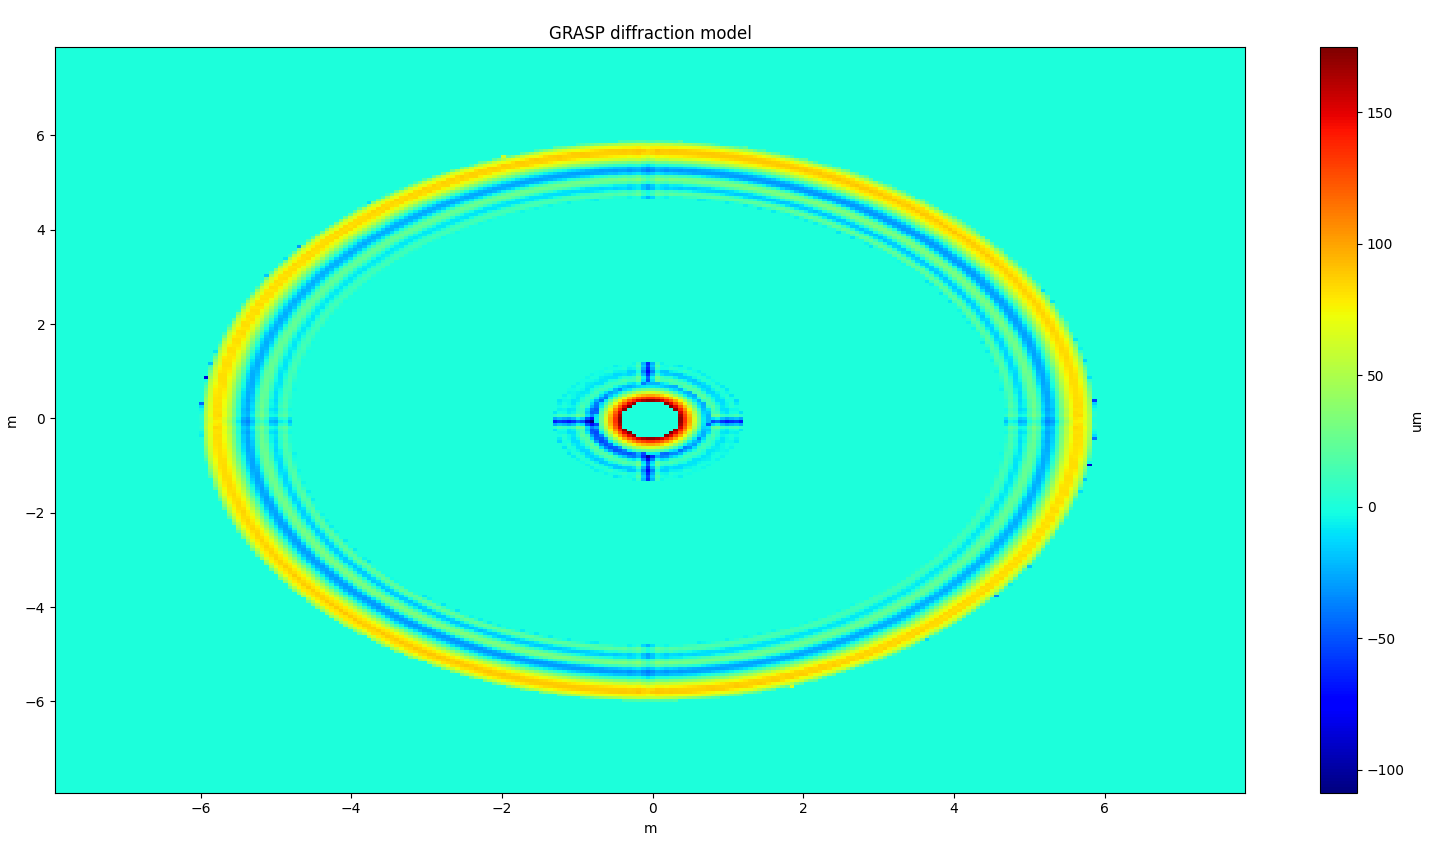
\includegraphics[width=0.8\textwidth]{images/grasp_diffraction_model.png}
    \caption{GRASP diffraction model.}
    \label{fig:grasp_diffraction}
\end{figure}


\begin{figure}
    \centering
    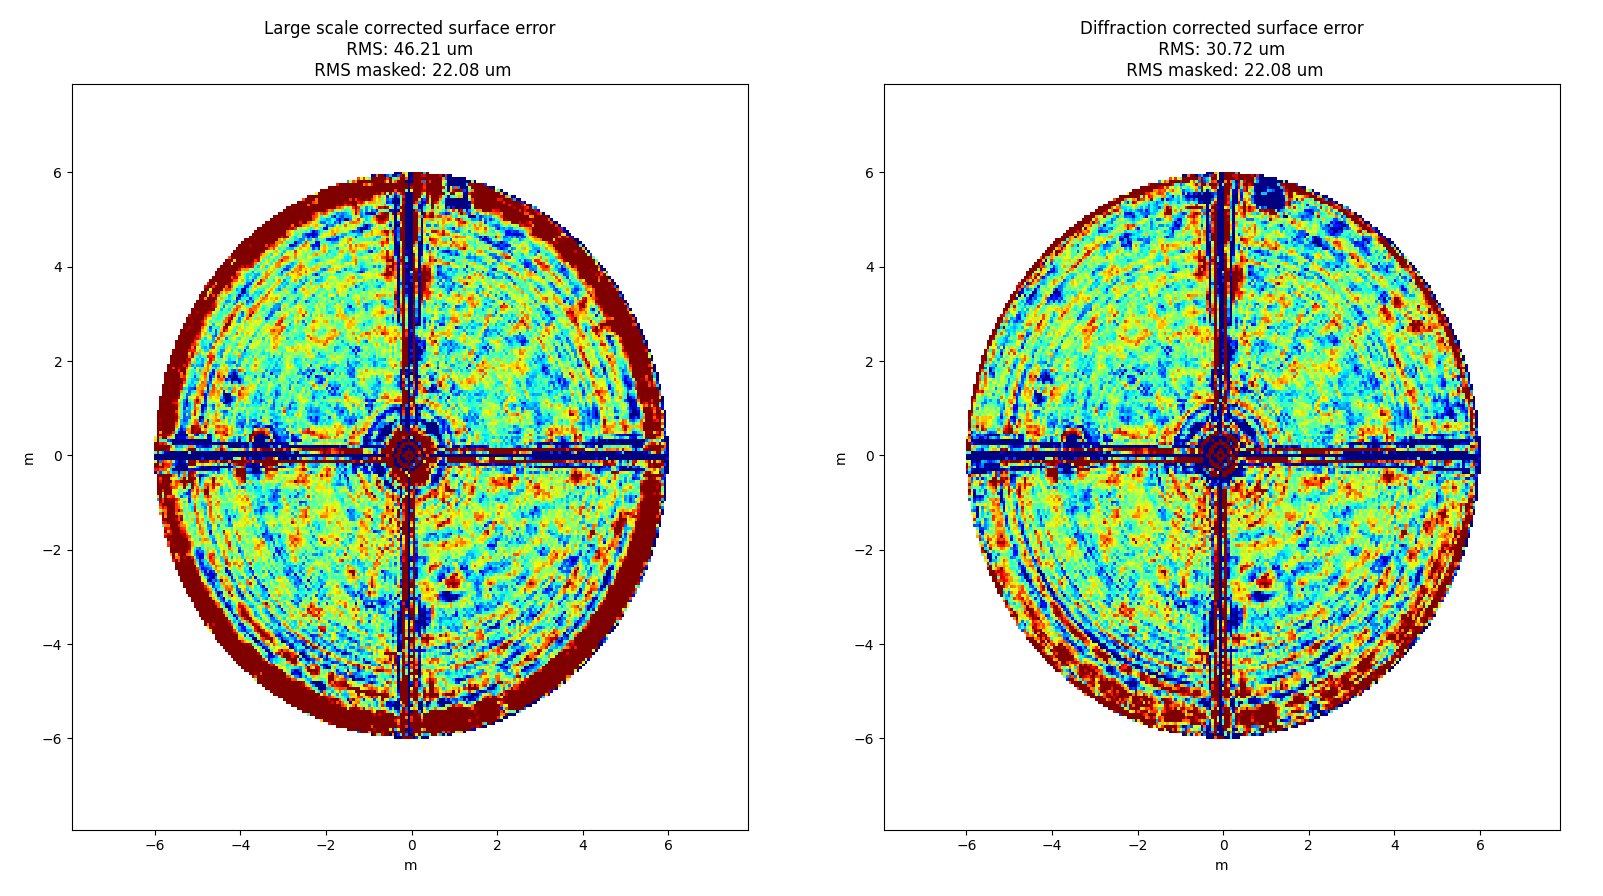
\includegraphics[width=0.9\textwidth]{images/diffraction_correction.png}
    \caption{Example of the effect of the substraction of the diffraction model.}
    \label{fig:diffraction_corrected}
\end{figure}



\subsection{Supporting legs substraction}

To account the effect on the supporting legs a more practical approach was taken. We devided the total radius of the dish in different zones, eg: $[0.375, 1.75, 3.,4.5, 6]$. Since we are going to assume axial symmetry along the vertical and horizontal axis, we separate the effect of the legs placed vertically and the ones placed horizontally.

As an example we are going to take the X axis and the radius region $[0.375, 1.75[$ and considering the legs width as $0.4m$, we have two regions to consider: the one at $A1=(-1.75,0.2), (-0.375,0.2), (-0.375, -0.2), (-1.75,-0.2)$ and $A2=(0.375,0.2), (1.75, 0.2), (1.75, -0.2), (0.375,-0.2)$ as show in the figure \ref{fig:ex_legs_region}. As this example is in the X axis, we will move in the Y direction and for each Y value we will compute the median (or average) of the pixels at that heigh (from both regions $A1$ and $A2$) and this value will be the correction for all the pixels at that height.


For the case of Y axis, the median (or average) computation will be at each X value.
The figure \ref{fig:legs_removal} shows the final model result and the effect iof its substraction, the input map used to obtain these figures is the same one obtained from the diffraction model correction shown in \ref{fig:diffraction_corrected}.

\begin{figure}
    \centering
    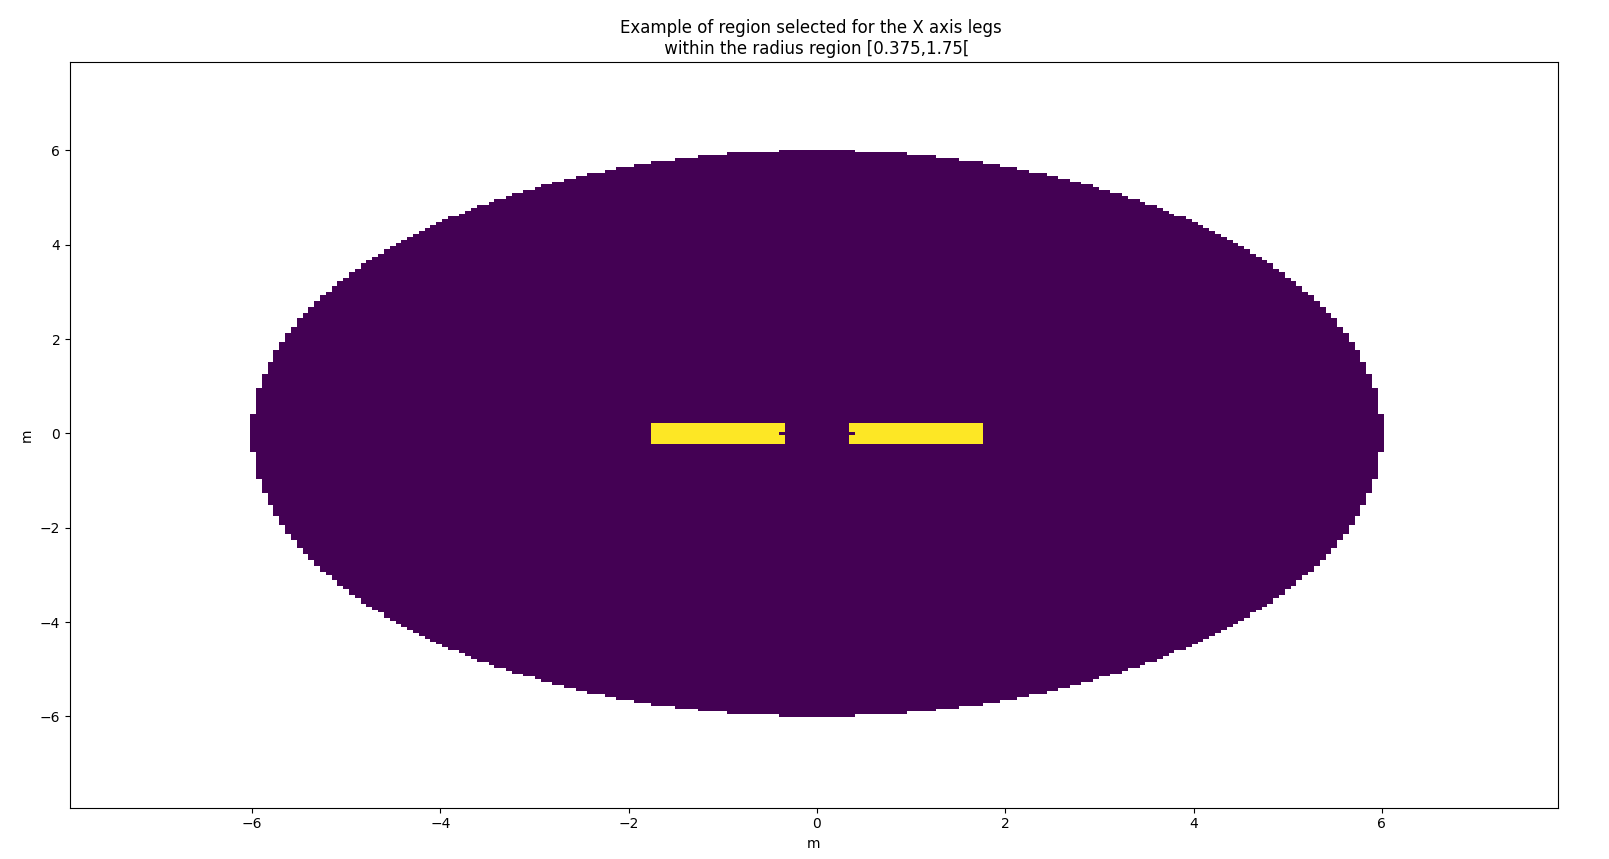
\includegraphics[width=0.9\textwidth]{images/ex_legs_region.png}
    \caption{Example of the regions selected for X axis supporting legs within the radius $[0.375,1.75[$.}
    \label{fig:ex_legs_region}
\end{figure}


\begin{figure}
    \centering
    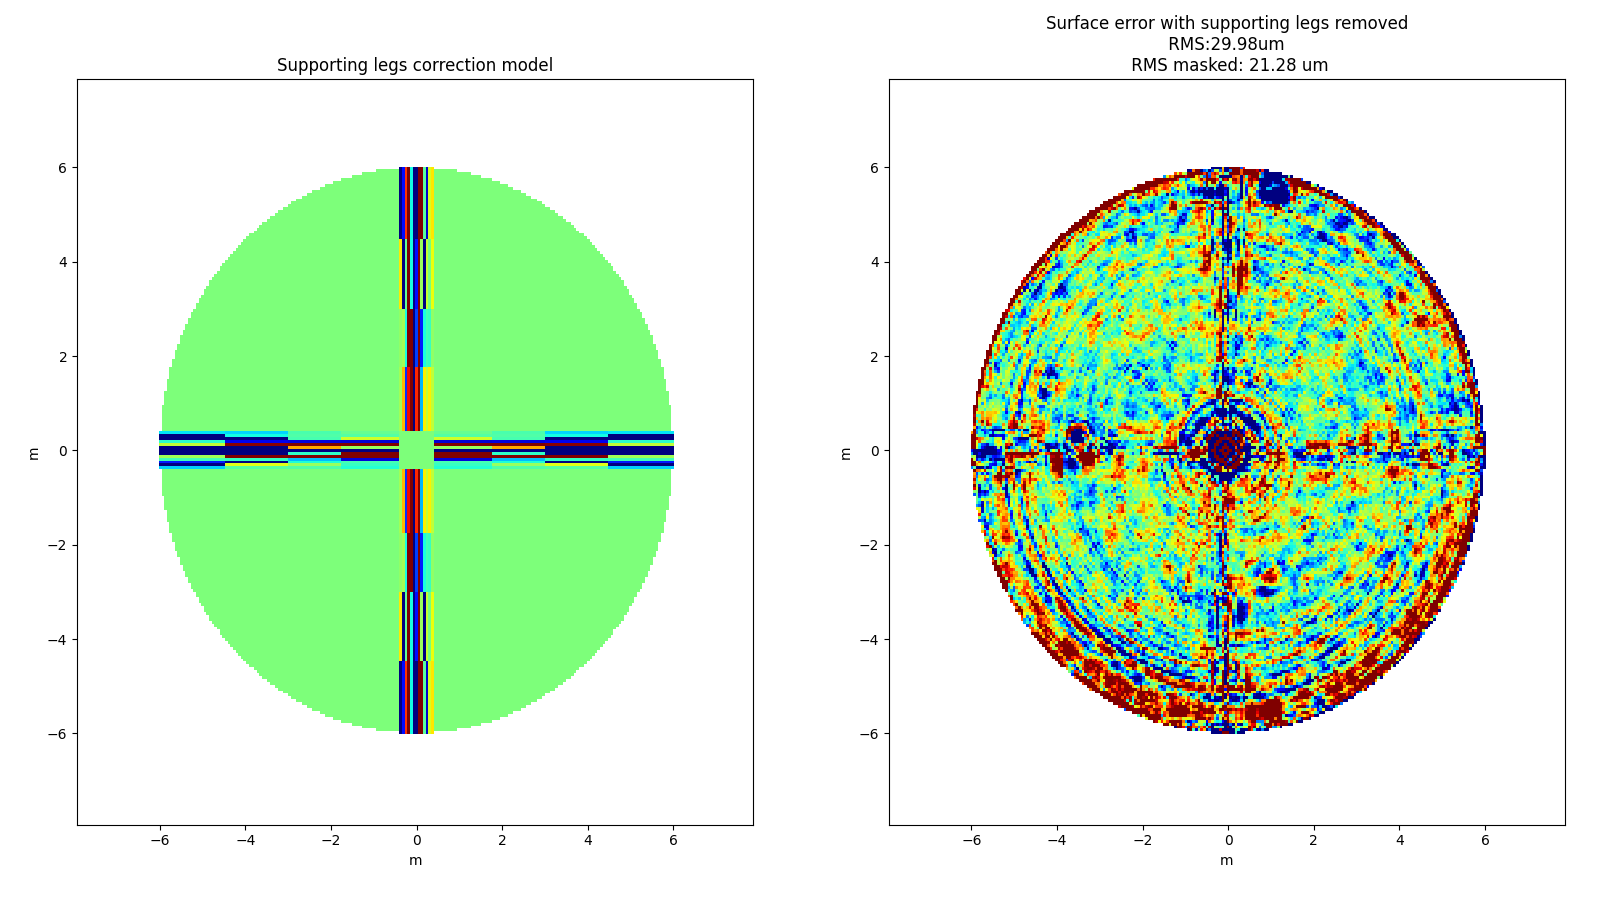
\includegraphics[width=0.9\textwidth]{images/legs_removal.png}
    \caption{Supporting legs model and the resulf of its removal in the surface error map.}
    \label{fig:legs_removal}
\end{figure}






